\section{M2T Transformation with XPand}
\label{appendix.xpand}

\begin{figure}[H]
	\centering
	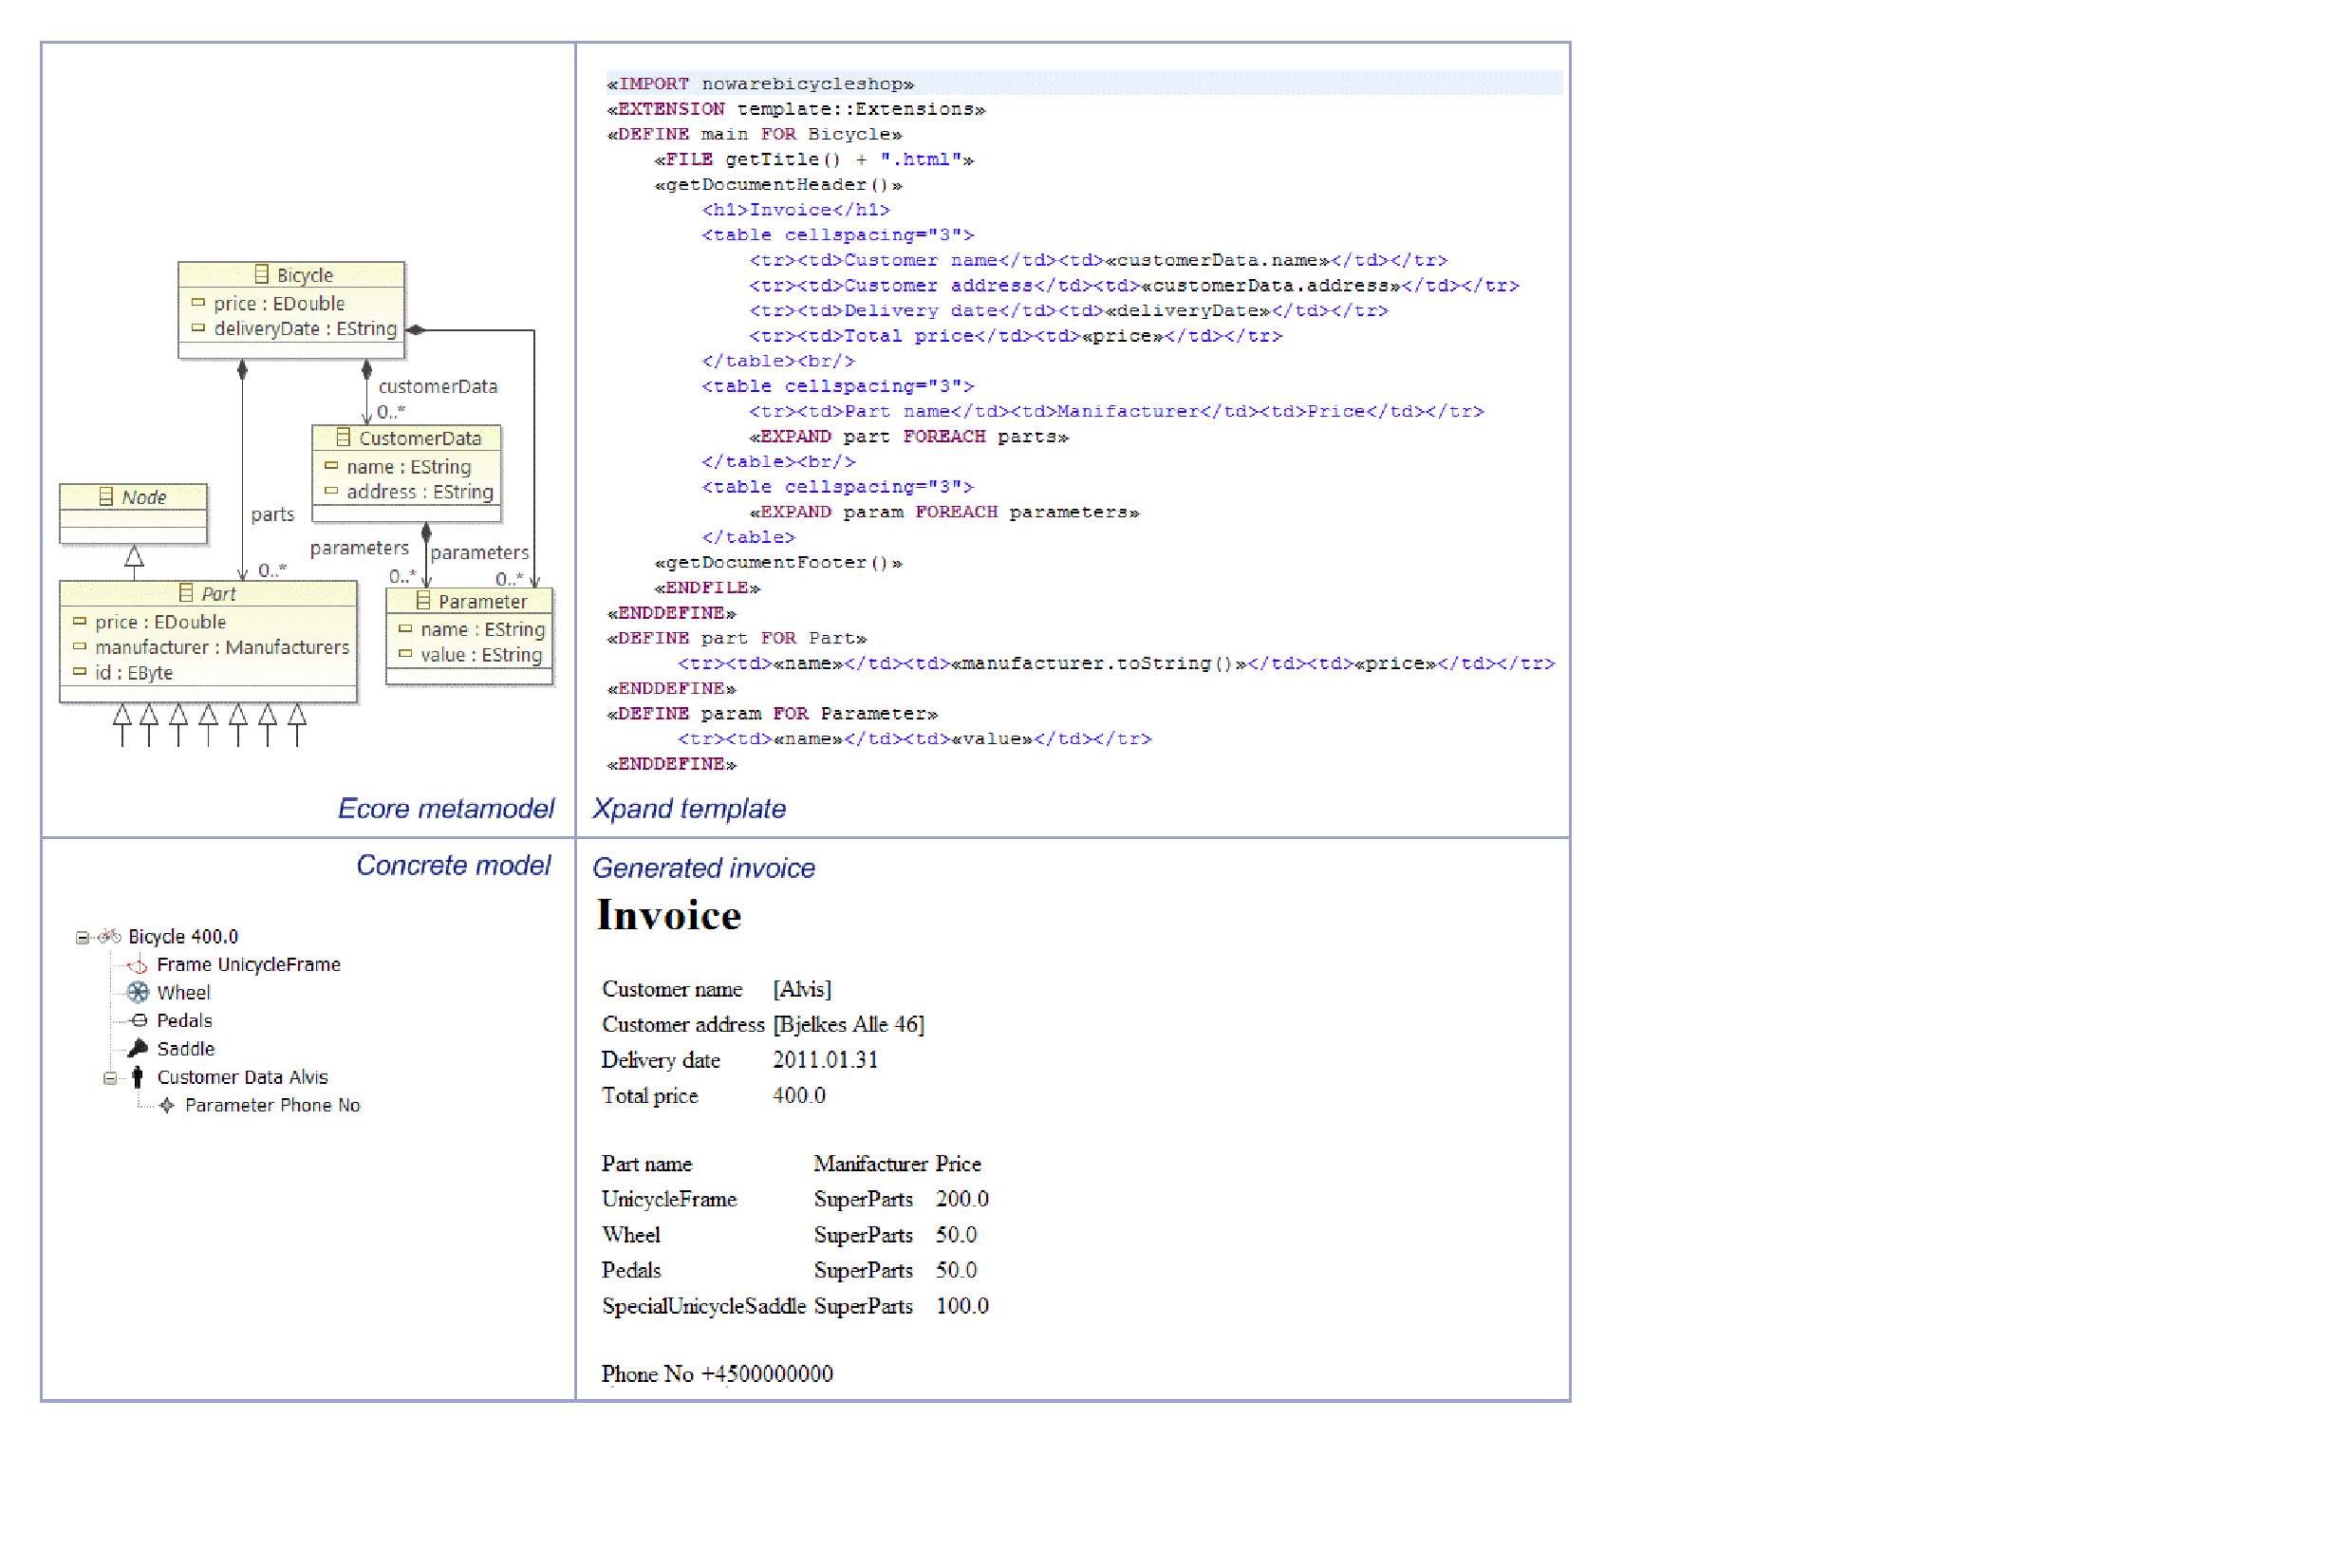
\includegraphics[width=1.0\linewidth]{fig/xpand/model_xpand_invoice.pdf}
	\caption{The InvoiceTemplate and a generated invoice examle}
	\label{fig.xpand.model_xpand_invoice}
\end{figure}

\clearpage

\begin{figure}[htp]
	\centering
	\subfigure[]{
		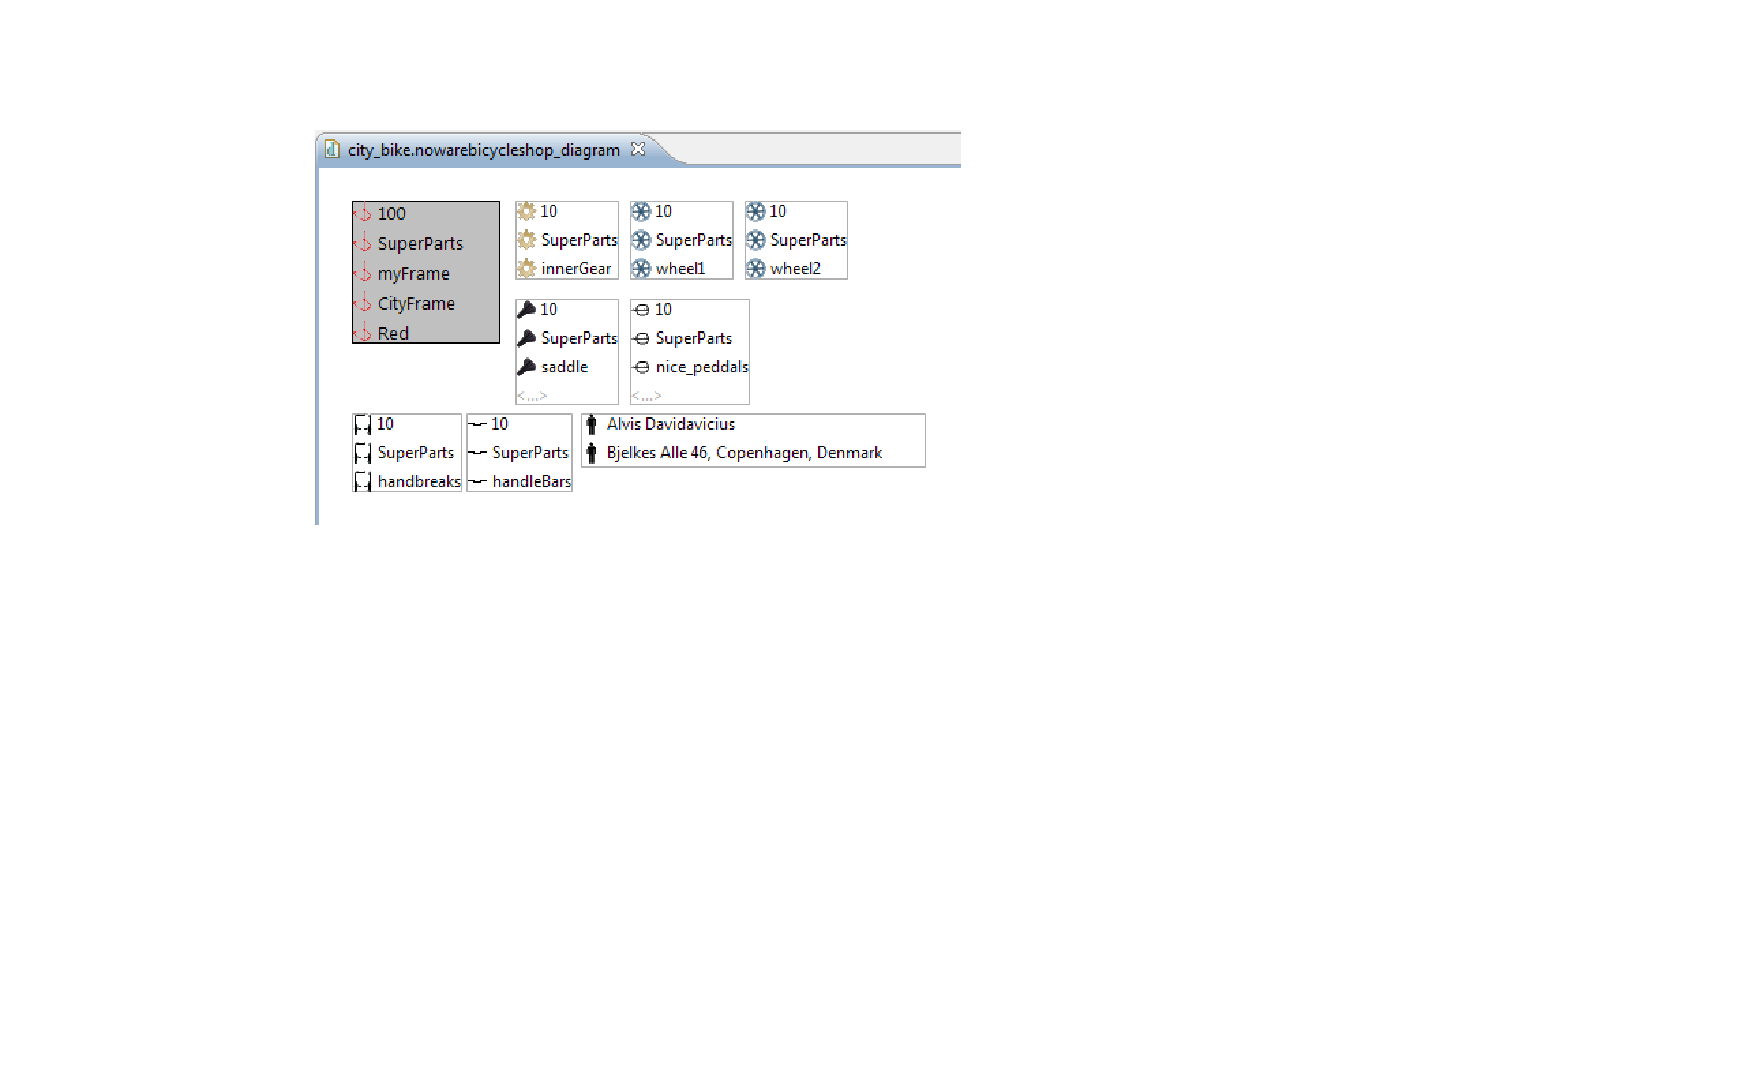
\includegraphics[width=0.3\linewidth]{fig/xpand/usecase/s1.pdf}
	}
	\subfigure[]{
		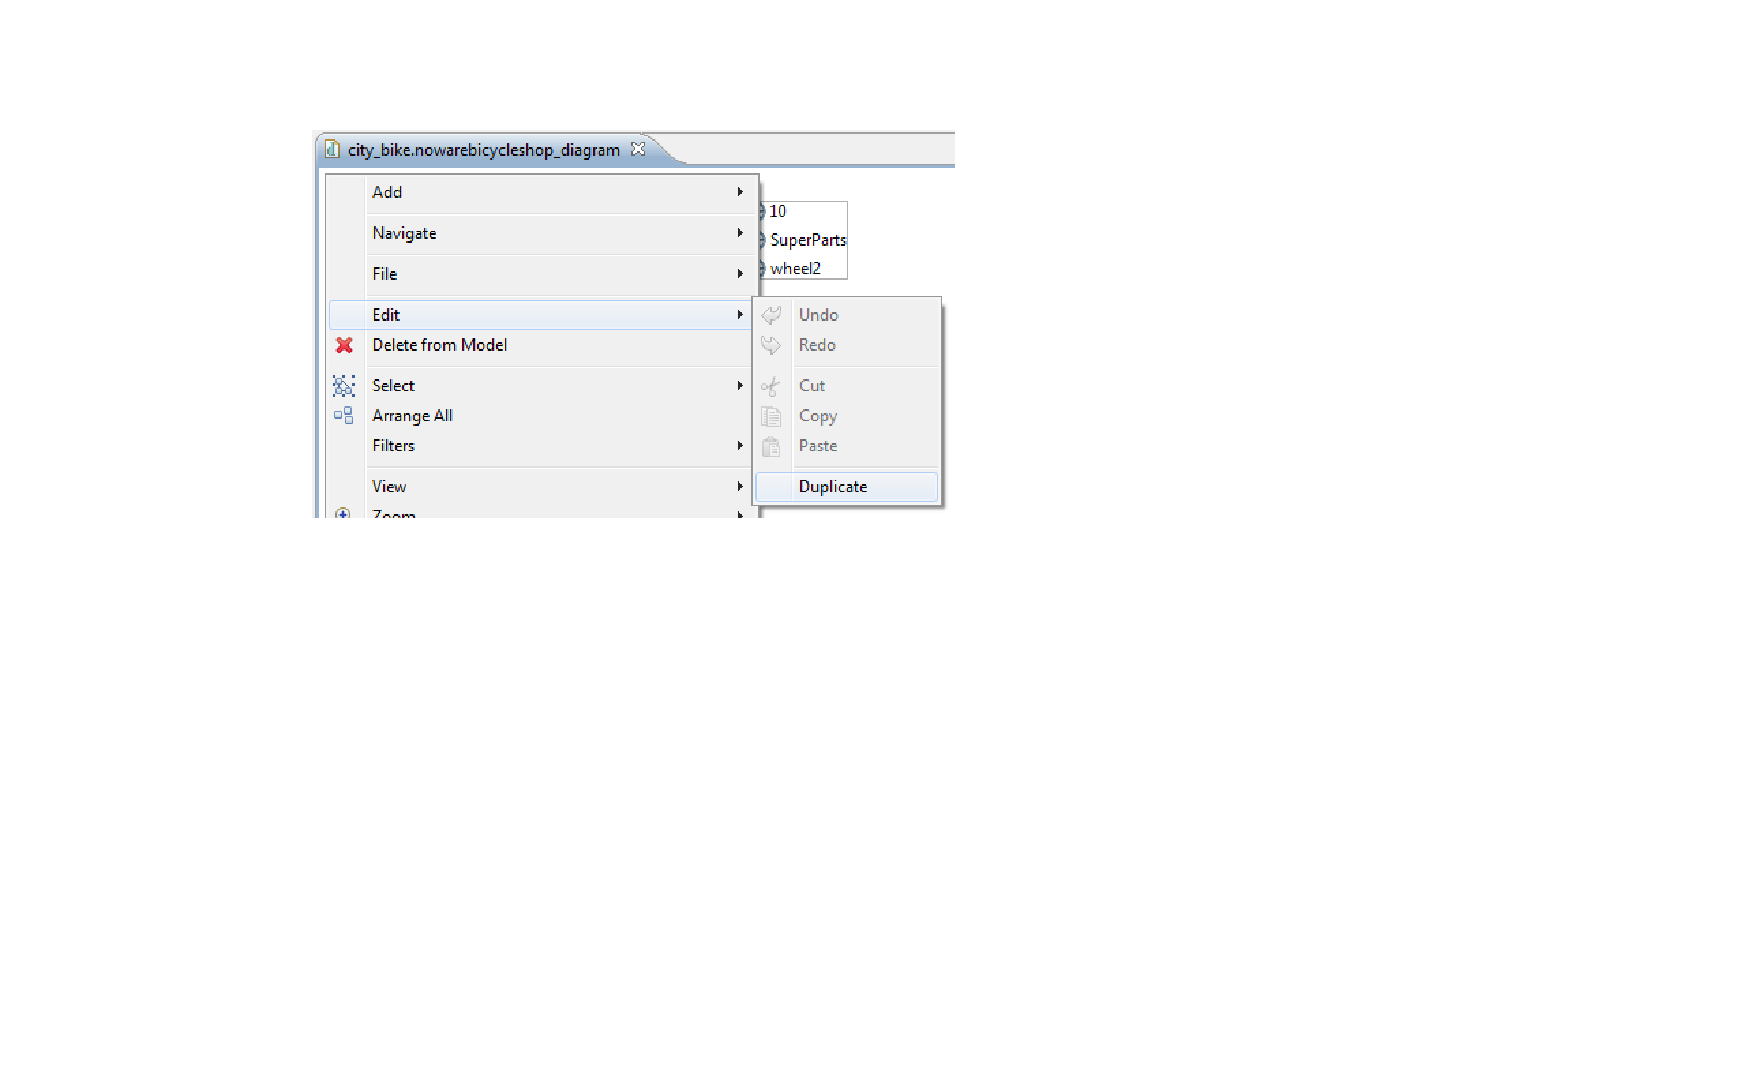
\includegraphics[width=0.3\linewidth]{fig/xpand/usecase/s2.pdf}
	}
	\subfigure[]{
		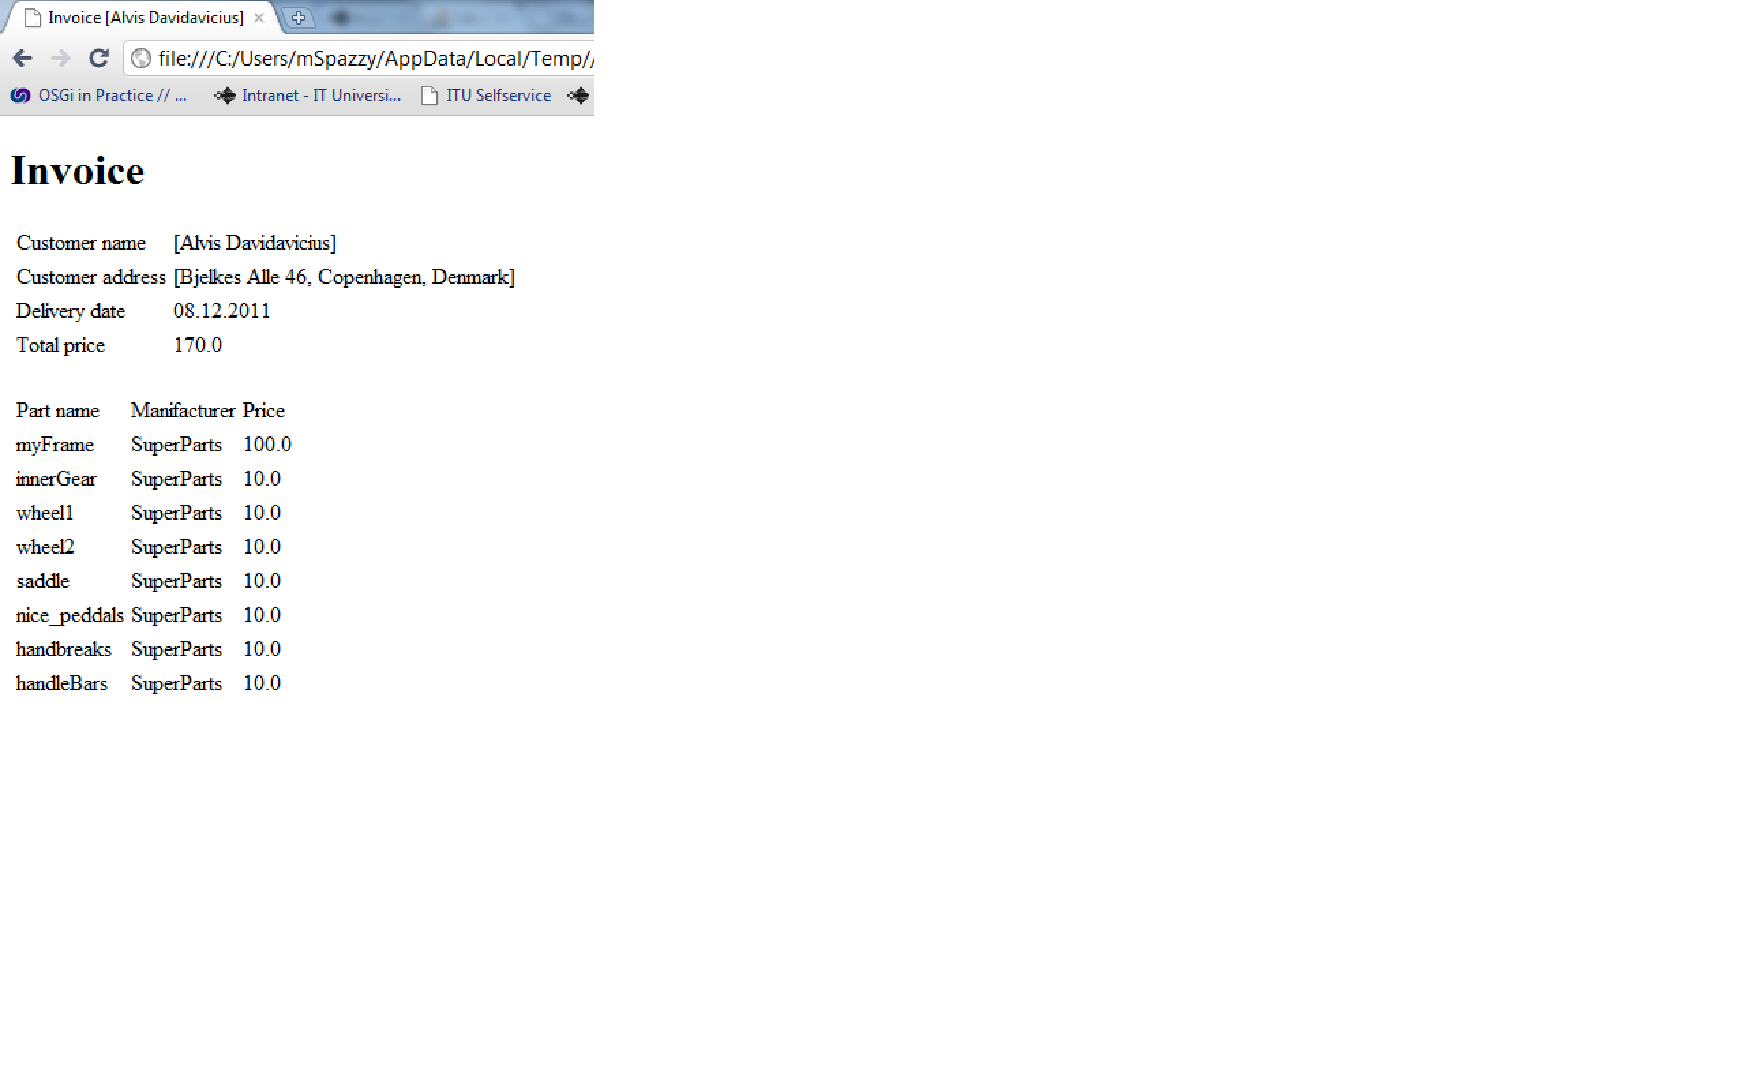
\includegraphics[width=0.3\linewidth]{fig/xpand/usecase/s3.pdf}
	}
	\caption{Invoking invoice generation}
	\label{fig.xpand.usecase}
\end{figure}

\subsection{Implementation}
\label{appendix.xpand.implementation}

\begin{center}
	\lstset{captionpos=b,language=Java,numbers=none,basicstyle=\small}
	\lstset{linewidth=1.0\textwidth}
	\lstset{
keywordstyle=\bfseries\ttfamily\color[rgb]{0,0,1},
identifierstyle=\ttfamily,
commentstyle=\color[rgb]{0.133,0.545,0.133},
stringstyle=\ttfamily\color[rgb]{0.627,0.126,0.941},
showstringspaces=false,
basicstyle=\small,
numbers=none,
stepnumber=1,
numbersep=10pt,
tabsize=2,
breaklines=true,
prebreak = \raisebox{0ex}[0ex][0ex]{\ensuremath{\hookleftarrow}},
breakatwhitespace=false,
aboveskip={1.5\baselineskip},
columns=fixed,
upquote=true,
extendedchars=true,
}

\lstset{label=lst.extensions,caption=Extensions.ext}
\lstinputlisting{appendix/src_code/Extensions.in}

\lstset{label=edit_policy_provider,caption=EditPolicyProvider.java}
\lstinputlisting{appendix/src_code/EditPolicyProvider.in}

\lstset{label=open_edit_policy,caption=OpenEditPolicy.java}
\lstinputlisting{appendix/src_code/OpenEditPolicy.in}
\end{center}